%!TEX root = <main.tex>
\appendix

\section{Special Situations with Incremental Inference}

\begin{figure}[t]
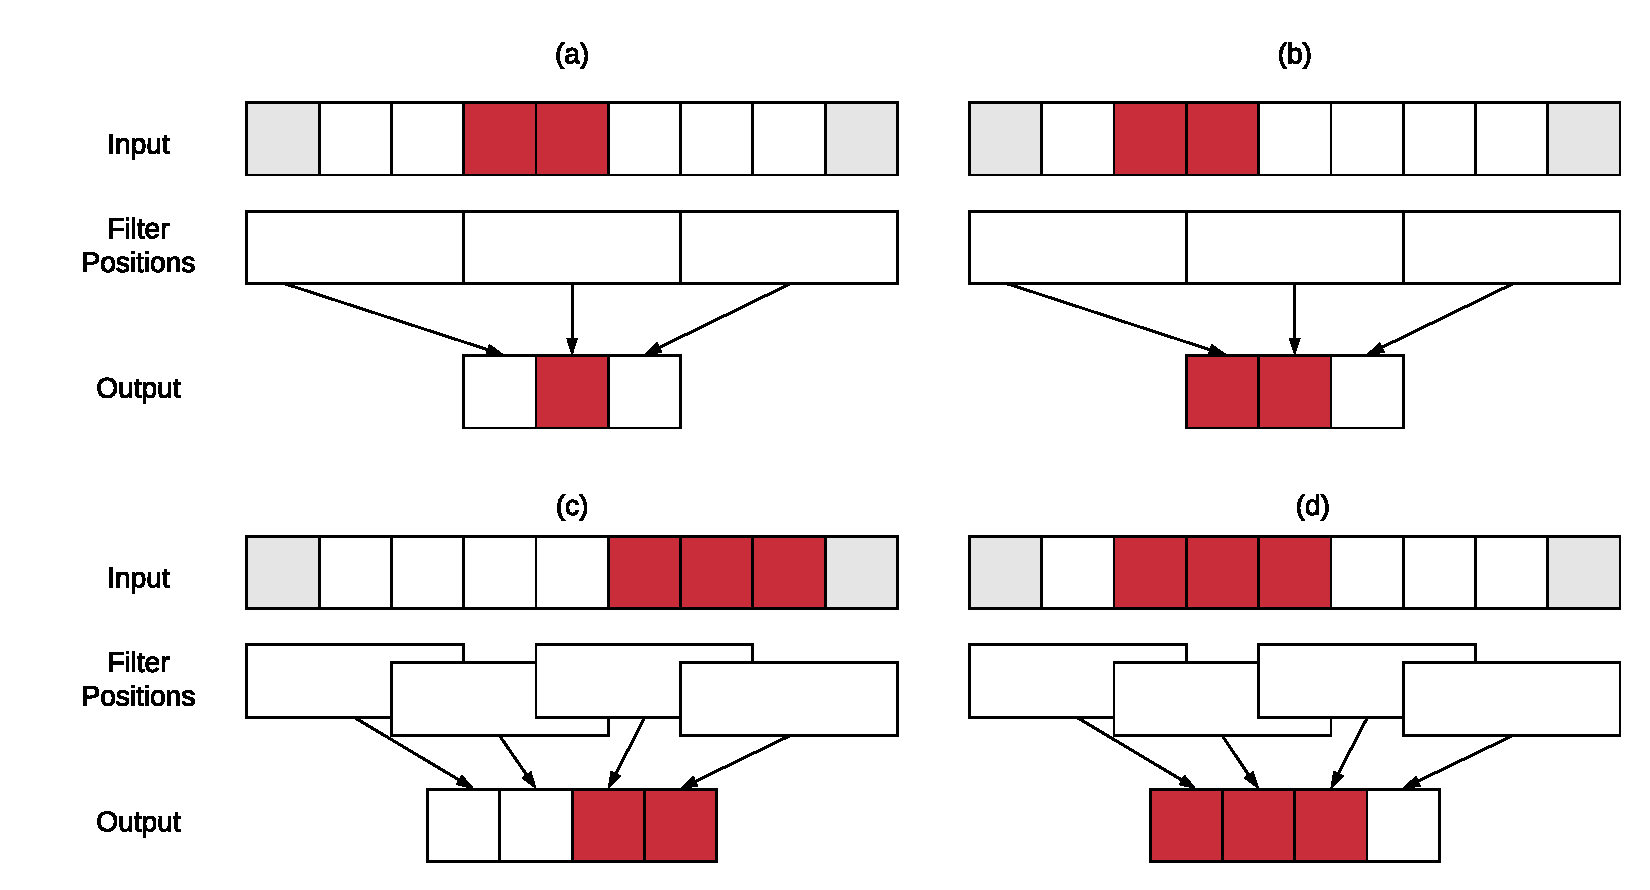
\includegraphics[width=\columnwidth]{images/less_one_example}
\caption{One dimensional representation showing special situations under which actual output size will be smaller than the values calculated by Equations \ref{eqn:xcoordinate} and \ref{eqn:ycoordinate}. (a) and (b) shows a situation with filter stride being equal to the filter size. (c) and (d) shows a situation with input patch being placed at the edge of the input.}
\label{fig:less_one_example}
\end{figure}

It is important to note that there are special situations under which the actual output patch size can be smaller than the values calculated in Section \ref{sec:inc_computation}. Consider the simplified one dimensional situation shown in Figure \ref{fig:less_one_example} (a), where the stride value\footnote{Note that the stride value is generally less than or equal to the filter size.} (3) is same as the filter size (3). In this situation the the size of the output patch is one less than the value calculated by Equation \ref{eqn:patchwidth}. However it is not the case in Figure \ref{fig:less_one_example} (b) which has the same input patch size but is placed at a different location.
% This issue arises only when the stride value is same as the filter size.
Another situation arises when the input patch is placed at the edge of the input as shown in Figure \ref{fig:less_one_example} (c). In this situation it is not possible for the filter to move freely through all filter positions as it hits the input boundary compared to having the input patch on the middle of the input as shown in Figure \ref{fig:less_one_example} (c).
In \system~ we do not treat theses differences separately and use the values calculated by Equation \ref{eqn:patchwidth} and \ref{eqn:patchheight} as they act as an upper bound. In case of a smaller output patch, \system~ simply reads off and updates slightly bigger patches to preserve uniformity.
This also requires updating the starting coordinates of the patches as shown in Equations \ref{eqn:width_subtract} and \ref{eqn:height_subtract}.
Such uniform treatment is required for performing batched inference operations which out of the box gives significant speedups compared to per image inference.

\vspace{2mm}
\hspace{4mm} If $x^\mathcal{O}_\mathcal{P} + W^\mathcal{O}_\mathcal{P} > W_{\mathcal{O}}:$
\begin{align}
\begin{split}
\label{eqn:width_subtract}
x^\mathcal{O}_\mathcal{P} = &~ W_{\mathcal{O}} - W^\mathcal{O}_\mathcal{P}\\
x^\mathcal{I}_\mathcal{P} = &~ W_{\mathcal{I}} - W^\mathcal{I}_\mathcal{P}\\
x^\mathcal{R}_\mathcal{P} = &~ W_{\mathcal{I}} - W^\mathcal{R}_\mathcal{P}
\end{split}
\end{align}

\hspace{4mm} If $y^\mathcal{O}_\mathcal{P} + H^\mathcal{O}_\mathcal{P} > H_{\mathcal{O}}:$
\begin{align}
\begin{split}
\label{eqn:height_subtract}
y^\mathcal{O}_\mathcal{P} = &~ H_{\mathcal{O}} - H^\mathcal{O}_\mathcal{P}\\
y^\mathcal{I}_\mathcal{P} = &~ H_{\mathcal{I}} - H^\mathcal{I}_\mathcal{P}\\
y^\mathcal{R}_\mathcal{P} = &~ H_{\mathcal{I}} - H^\mathcal{R}_\mathcal{P}
\end{split}
\end{align}

\section{Fine-tuning CNNs}

For \textit{OCT} and \textit{Chest X-Ray} datasets the three ImageNet pre-trained CNN models are fine-tuned by retraining the final layer.
We use a train-validation-test split of 60-20-20 and the exact numbers for each dataset are shown in Table \ref{tbl:dataset_sizes}.
Cross-entropy loss with L2 regularization is used as the loss function and  Adam \cite{kingma2014adam} is used as the optimizer.
We tune learning rate $\eta \in [10^{-2}, 10^{-4}, 10^{-6}]$ and regularization parameter $\lambda \in [10^{-2}, 10^{-4}, 10^{-6}]$ using the validation set and train for 25 epochs.
Table \ref{tbl:finetune_accuracies} shows the final train and test accuracies.

\begin{table}[ht]
\begin{tabular}{|l|l|l|l|}
\hline
\multirow{2}{*}{} & \multicolumn{1}{c|}{\multirow{2}{*}{Train}} & \multicolumn{1}{c|}{\multirow{2}{*}{Validation}} & \multicolumn{1}{c|}{\multirow{2}{*}{Test}} \\
 & \multicolumn{1}{c|}{} & \multicolumn{1}{c|}{} & \multicolumn{1}{c|}{} \\ \hline
OCT & 50,382 & 16,853 & 16, 857 \\ \hline
Chest X-Ray & 3,463 & 1,237 & 1,156 \\ \hline
\end{tabular}
\caption{Train-validation-test split size for each dataset.}
\label{tbl:dataset_sizes}
\end{table}

\begin{table}[ht]
\begin{tabular}{|c|l|l|l|l|l|l|}
\hline
\multicolumn{1}{|l|}{\multirow{3}{*}{}} & \multirow{3}{*}{Model} & \multicolumn{2}{l|}{\multirow{2}{*}{Accuracy(\%)}} & \multicolumn{3}{l|}{\multirow{2}{*}{Hyperparams.}} \\
\multicolumn{1}{|l|}{} &  & \multicolumn{2}{l|}{} & \multicolumn{3}{l|}{} \\ \cline{3-7} 
\multicolumn{1}{|l|}{} &  & Train & Test & \multicolumn{2}{l|}{$\eta$} & $\lambda$ \\ \hline
\multirow{3}{*}{OCT} & VGG16 & 79 & 82 & \multicolumn{2}{l|}{$10^{-4}$} & $10^{-4}$ \\ \cline{2-7} 
 & ResNet18 & 79 & 82 & \multicolumn{2}{l|}{$10^{-2}$} & $10^{-4}$ \\ \cline{2-7} 
 & Inception3 & 71 & 81 & \multicolumn{2}{l|}{$10^{-2}$} & $10^{-6}$ \\ \hline
\multirow{3}{*}{Chest X-Ray} & VGG16 & 75 & 76 & \multicolumn{2}{l|}{$10^{-4}$} & $10^{-4}$ \\ \cline{2-7} 
 & ResNet18 & 78 & 76 & \multicolumn{2}{l|}{$10^{-4}$} & $10^{-6}$ \\ \cline{2-7} 
 & Inception3 & 74 & 76 & \multicolumn{2}{l|}{$10^{-4}$} & $10^{-2}$ \\ \hline
\end{tabular}
\caption{Train and test accuracies after fine-tuning.}
\label{tbl:finetune_accuracies}
\end{table}

\section{Visual Examples}

Figure \ref{fig:visual_examples} presents occlusion heatmaps for a sample image from each dataset with (a) \textit{incremental inference} and (b) \textit{incremental inference} with \textit{adaptive drill-down} for different \textit{projective field threshold} values. The predicted class label for \textit{OCT}, \textit{Chest X-Ray}, and \textit{ImageNet} are DME, VIRAL, and OBOE respectively.

\begin{figure*}[t]
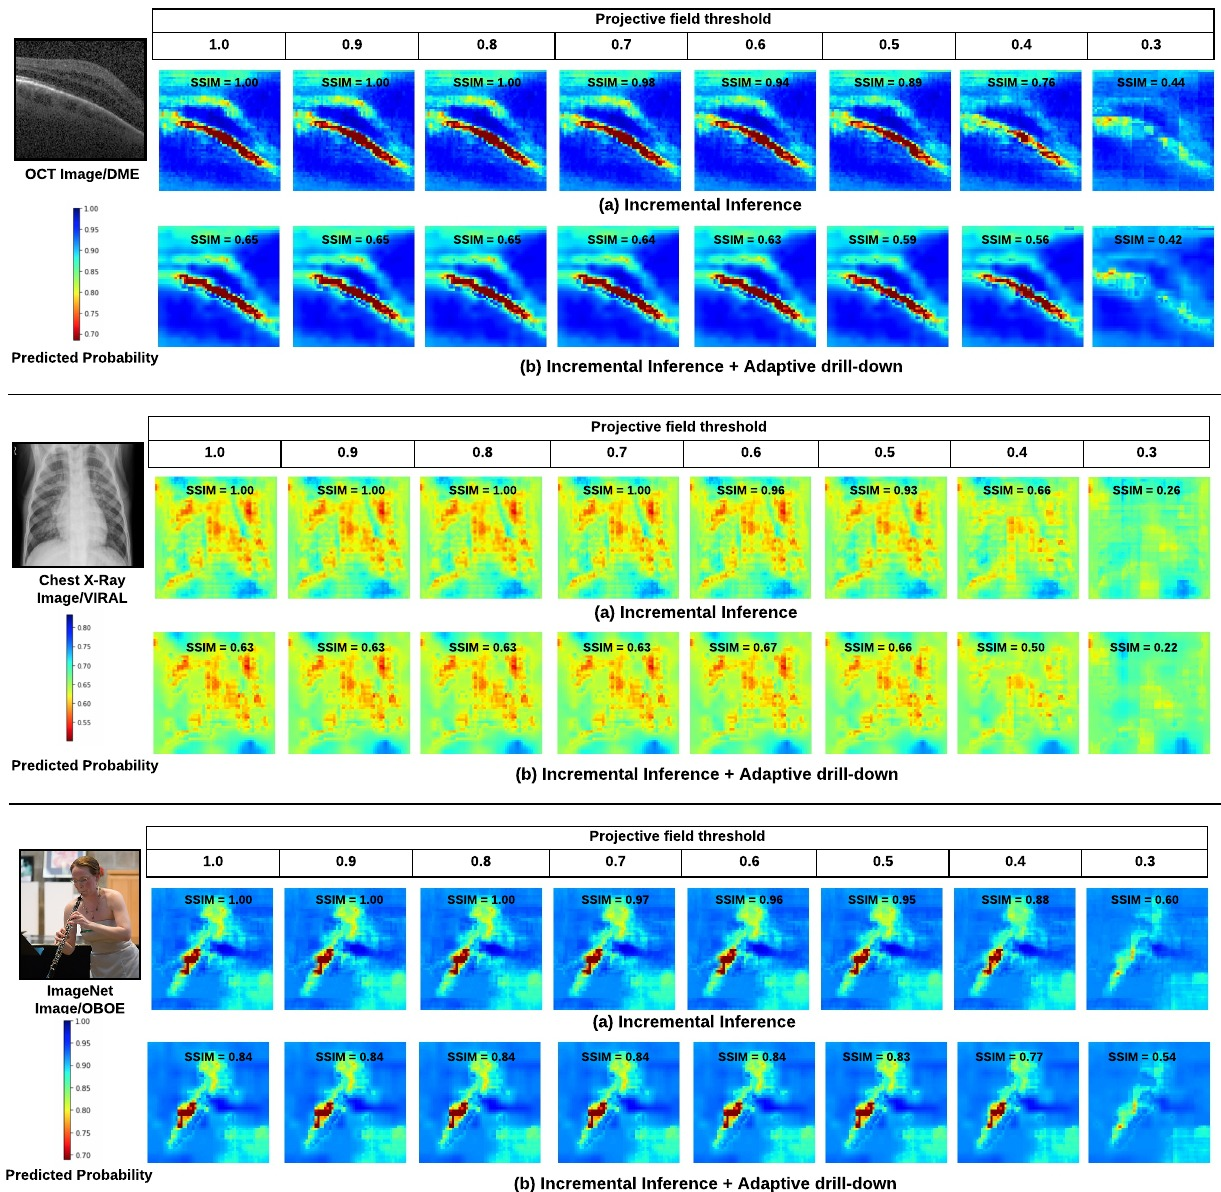
\includegraphics[width=\textwidth]{images/visual_examples}
\caption{Occlusion heatmaps for sample images (CNN model = VGG16, occlusion patch size = 16, patch color = black, occlusion patch stride $(S~or~S_2)$ = 4. For \textit{OCT} $r_{drill\_down}=0.1$ and target \texttt{speedup}=5. For \textit{Chest X-Ray} $r_{drill\_down}=0.4$ and target \texttt{speedup}=2. For \textit{ImageNet} $r_{drill\_down}=0.25$ and target \texttt{speedup}=3).}
\label{fig:visual_examples}
\end{figure*}

